%%%%%%%%%%%%%%%%%%%%%%%%%%%%%%%%%%%%%%%%%%%%%%%%%%%%%%%%%%%%%%%%%%
%%%%%%%% ICML 2013 EXAMPLE LATEX SUBMISSION FILE %%%%%%%%%%%%%%%%%
%%%%%%%%%%%%%%%%%%%%%%%%%%%%%%%%%%%%%%%%%%%%%%%%%%%%%%%%%%%%%%%%%%

% Use the following line _only_ if you're still using LaTeX 2.09.
%\documentstyle[icml2013,epsf,natbib]{article}
% If you rely on Latex2e packages, like most moden people use this:
\documentclass{article}

% For figures
\usepackage{graphicx} % more modern
%\usepackage{epsfig} % less modern
\usepackage{subfigure} 

% For citations
\usepackage{natbib}

% For algorithms
\usepackage{algorithm}
\usepackage{algorithmic}

% As of 2011, we use the hyperref package to produce hyperlinks in the
% resulting PDF.  If this breaks your system, please commend out the
% following usepackage line and replace \usepackage{icml2013} with
% \usepackage[nohyperref]{icml2013} above.
\usepackage{hyperref}

% Packages hyperref and algorithmic misbehave sometimes.  We can fix
% this with the following command.
\newcommand{\theHalgorithm}{\arabic{algorithm}}

% Employ the following version of the ``usepackage'' statement for
% submitting the draft version of the paper for review.  This will set
% the note in the first column to ``Under review.  Do not distribute.''
\usepackage{icml2013} 
% Employ this version of the ``usepackage'' statement after the paper has
% been accepted, when creating the final version.  This will set the
% note in the first column to ``Proceedings of the...''
% \usepackage[accepted]{icml2013}


% The \icmltitle you define below is probably too long as a header.
% Therefore, a short form for the running title is supplied here:
\icmltitlerunning{Building Multi-Class Models with the Iris Dataset}

\begin{document} 

\twocolumn[
\icmltitle{Building Multi-Class Models with the Iris Dataset}

% It is OKAY to include author information, even for blind
% submissions: the style file will automatically remove it for you
% unless you've provided the [accepted] option to the icml2013
% package.
\icmlauthor{Carl Cortright}{carl.cortright@colorado.edu}
\icmladdress{University of Colorado Boudler}
\icmlauthor{Your CoAuthor's Name}{email@coauthordomain.edu}

% You may provide any keywords that you 
% find helpful for describing your paper; these are used to populate 
% the "keywords" metadata in the PDF but will not be shown in the document
\icmlkeywords{boring formatting information, machine learning, ICML}

\vskip 0.3in
]

\section{Introduction} 

One of the classic example data sets in machine learning is the Iris dataset. This dataset contains three different species of iris, each entry with a measurement of sepal length and width and pedal length and width. For this project, I split the Iris dataset in to two, one for testing and one for training. Then, I trained two different models, one using a custom naive bayes algorithm and the other using vowpal wabbit. Later we compare the two models for accuracy and explain some flaws in our experiment. 
  

\section{Naive Bayes Analysis}

\subsection{Experimental Setup}

For this experiment, I used a python script to train a model on various sized datasets. Then, using the rest of the iris model, I tested for accuracy. I also used basic "Add 1" smoothing to account for features that weren't seen in training.  The naive bayes algorithm used, uses log space multiplication to simplify the expression\\

$P(C) \prod_{i=0}^n P(X_i | C) = log(P(C)) + log(P(X_0|C)) + ... + log(P(X_n|C)$

\subsection{Results}

Shuffling the dataset between runs, I computed the accuracy based on different ratios of training:test data. With ratios ranging from 1:1 to 15:1 , I ran 5000 tests on each ratio to calculate the average accuracy, producing figure 1.

\begin{figure}[!ht]

\caption{The blue line represents best fit, and the ratio is the number on the x-axis:1 (training:test)}
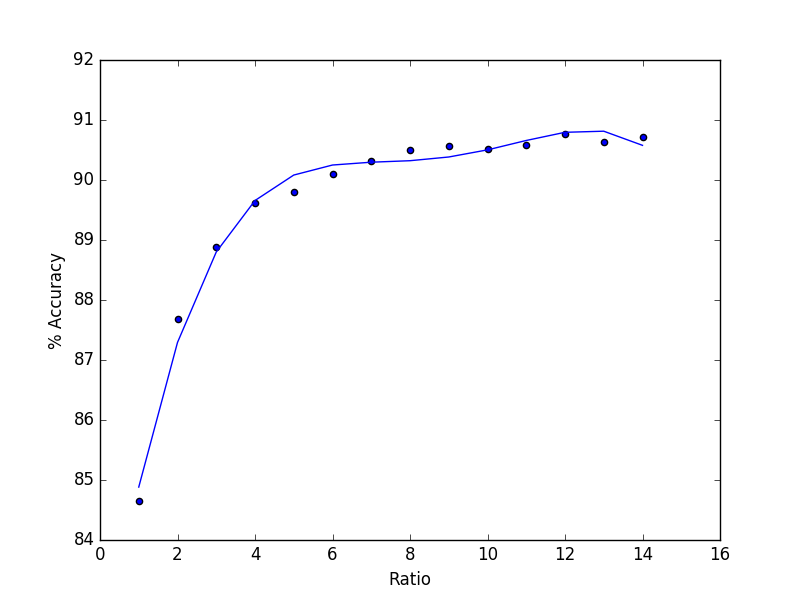
\includegraphics[width=\columnwidth]{figure_1.png}

\end{figure}

As expected, the larger the training set, the more accurate the model. As we approach the full size of the dataset, the accuracy appears to approach somewhere around 91 percent, a decent result for naive bayes. With a larger dataset, the accuracy could likely be increased. 

\section{Vowpal Wabbit Analysis}

\subsection{Experimental Setup}

To set up VW, I shuffled the iris dataset and put it in two separate files, one for training and one for testing. Then, I used the scripts given to us to train and test the dataset using vowpal wabbit. Afterwards, I used a custom python script to calculate the accuracy of the model.


\subsection{Results}

After training my model with VW, I was able to get an accuracy of 100 percent using a similar ratio to that used in the naive bayes model. This makes sense, a model like vowpal wabbit that uses logistic regression rather than naive bayes normally performs better.

\section{Conclusion}

For this project, I used the iris dataset to create two different multi-class models to predict flower type. Based on the experiments I ran, I determined that vowpal wabbit is a superior method to naive bayes for predicting class using this dataset. Overall, our predictions weren't very accurate. We did show that the more training examples, the better the model that resulted. In order to create a more robust system with either method, we would likely need a larger dataset to train on. 


\section{Software and Data}

Vowpal Wabbit\\ https://github.com/JohnLangford/vowpal_wabbit\\
Iris Dataset\\ https://archive.ics.uci.edu/ml/datasets/Iris\\


% In the unusual situation where you want a paper to appear in the
% references without citing it in the main text, use \nocite
\nocite{langley00}


\end{document} 


% This document was modified from the file originally made available by
% Pat Langley and Andrea Danyluk for ICML-2K. This version was
% created by Lise Getoor and Tobias Scheffer, it was slightly modified  
% from the 2010 version by Thorsten Joachims & Johannes Fuernkranz, 
% slightly modified from the 2009 version by Kiri Wagstaff and 
% Sam Roweis's 2008 version, which is slightly modified from 
% Prasad Tadepalli's 2007 version which is a lightly 
% changed version of the previous year's version by Andrew Moore, 
% which was in turn edited from those of Kristian Kersting and 
% Codrina Lauth. Alex Smola contributed to the algorithmic style files.  
